\documentclass{article}

\usepackage{tikz} 
\usetikzlibrary{automata, positioning, arrows} 

\usepackage{amsthm}
\usepackage{amsfonts}
\usepackage{amsmath}
\usepackage{amssymb}
\usepackage{fullpage}
\usepackage{color}
\usepackage{parskip}
\usepackage{hyperref}
\usepackage{graphicx}
  \hypersetup{
    colorlinks = true,
    urlcolor = blue,       % color of external links using \href
    linkcolor= blue,       % color of internal links 
    citecolor= blue,       % color of links to bibliography
    filecolor= blue,        % color of file links
    }
    
\usepackage{listings}
\usepackage[utf8]{inputenc}                                                    
\usepackage[T1]{fontenc}                                                       

\definecolor{dkgreen}{rgb}{0,0.6,0}
\definecolor{gray}{rgb}{0.5,0.5,0.5}
\definecolor{mauve}{rgb}{0.58,0,0.82}

\lstset{frame=tb,
  language=haskell,
  aboveskip=3mm,
  belowskip=3mm,
  showstringspaces=false,
  columns=flexible,
  basicstyle={\small\ttfamily},
  numbers=none,
  numberstyle=\tiny\color{gray},
  keywordstyle=\color{blue},
  commentstyle=\color{dkgreen},
  stringstyle=\color{mauve},
  breaklines=true,
  breakatwhitespace=true,
  tabsize=3
}

\newtheoremstyle{theorem}
  {\topsep}   % ABOVESPACE
  {\topsep}   % BELOWSPACE
  {\itshape\/}  % BODYFONT
  {0pt}       % INDENT (empty value is the same as 0pt)
  {\bfseries} % HEADFONT
  {.}         % HEADPUNCT
  {5pt plus 1pt minus 1pt} % HEADSPACE
  {}          % CUSTOM-HEAD-SPEC
\theoremstyle{theorem} 
   \newtheorem{theorem}{Theorem}[section]
   \newtheorem{corollary}[theorem]{Corollary}
   \newtheorem{lemma}[theorem]{Lemma}
   \newtheorem{proposition}[theorem]{Proposition}
\theoremstyle{definition}
   \newtheorem{definition}[theorem]{Definition}
   \newtheorem{example}[theorem]{Example}
\theoremstyle{remark}    
  \newtheorem{remark}[theorem]{Remark}

\title{CPSC-406 Report}
\author{Ethan Tapia  \\ Chapman University}

\date{\today} 

\begin{document}

\maketitle

\begin{abstract}
This report documents my journey through CPSC-406, focusing on the theoretical foundations of computation and algorithms. Beginning with the fundamentals of finite automata, the report progresses through deterministic and non-deterministic finite automata, regular expressions, context-free grammars, Turing machines, computability theory, and the complexity classes P and NP. Each section contains detailed solutions to weekly homework assignments, demonstrating my understanding and application of these concepts. The synthesis section explores the connections between complexity theory and practical algorithm design, while reflecting on the limitations of computational models. Throughout the course, I've developed not only technical skills in analyzing algorithms but also an appreciation for the elegant mathematical frameworks that underpin computer science.
\end{abstract}

\setcounter{tocdepth}{3}
\tableofcontents

\section{Introduction}\label{intro}
This report chronicles my semester-long exploration of the theoretical foundations of computer science in CPSC-406. The course has taken me from the basic building blocks of computation—finite automata and regular languages—to the frontiers of what computers can and cannot compute efficiently.

Beginning with deterministic finite automata (DFAs), I learned how to model simple computational processes and recognize regular languages. The progression to non-deterministic finite automata (NFAs) and their equivalence to DFAs demonstrated how different computational models can express the same language class. Regular expressions provided an elegant notation for describing patterns, while the subset construction and minimization algorithms revealed the practical aspects of implementing language recognizers.

As the course advanced, we explored more powerful computational models: context-free grammars, pushdown automata, and ultimately Turing machines. These models set the stage for understanding fundamental questions about computability—what problems can be solved algorithmically—and complexity—how efficiently such solutions can be implemented.

The analysis of algorithms formed a central theme, with asymptotic notation (Big O, Theta, Omega) providing a framework for comparing algorithm efficiency regardless of hardware specifics. The distinction between polynomial-time and exponential-time algorithms highlighted the practical importance of efficiency, while NP-completeness revealed a fascinating class of problems that resist efficient solutions despite their solutions being easily verifiable.

Network flow problems and Boolean satisfiability offered concrete examples of important computational problems with wide-ranging applications. The Ford-Fulkerson algorithm and SAT solvers demonstrated how theoretical concepts translate into practical algorithms for solving real-world problems.

Throughout this report, each weekly section documents not only the solutions to assigned problems but also my growing understanding of the theoretical landscape of computation. The synthesis section ties together these threads, reflecting on how this theoretical foundation informs my approach to algorithm design and analysis in practice.

\section{Week by Week}\label{homework}

\subsection{Week 1}
\textbf{Lecture Summary}

A finite automaton consists of a finite set of \textbf{states} ($Q$), an \textbf{alphabet} ($\Sigma$), a \textbf{transition function} ($\delta$), a \textbf{starting state} ($q_0$), and a set of \textbf{accepting states} ($F$). 

It can be formally represented as:

\[
M = (Q, \Sigma, \delta, q_0, F)
\]

where:
\begin{itemize}
    \item $Q$ is the set of states,
    \item $\Sigma$ is the input alphabet,
    \item $\delta: Q \times \Sigma \to Q$ is the transition function,
    \item $q_0 \in Q$ is the initial state,
    \item $F \subseteq Q$ is the set of accepting states.
\end{itemize}



\subsection{Week 2}
{\textbf{{Homework 1}}}

\textbf{Problem 1: Characterizing Accepted Sequences}

The given problem involves designing a finite automaton that accepts sequences of 5 and 10-cent inputs summing to 25 cents.

\textbf{Solution:}
We define the equation:
\begin{equation}
5a + 10b = 25
\end{equation}
where $a$ is the number of 5-cent inputs and $b$ is the number of 10-cent inputs. Solving for valid pairs:
\begin{itemize}
    \item $(a=5, b=0) \Rightarrow$ Sequence: $5,5,5,5,5$
    \item $(a=3, b=1) \Rightarrow$ Sequence: $5,5,5,10$
    \item $(a=1, b=2) \Rightarrow$ Sequence: $5,10,10$
\end{itemize}
These sequences are precisely those accepted by the automaton. The machine accepts a sequence if the total sum equals 25 cents.\newline

\textbf{Problem 2: Defining Valid Variable Names}

A valid variable name must begin with a letter ($\ell$) and be followed by any number of letters or digits ($d$).

\textbf{Regular Expression:}
\begin{equation}
\ell(\ell | d)^*
\end{equation}

\textbf{Solution:}
\textit{Finite Automaton:}
- States: $q_0$ (initial), $q_1$ (accepting).
- Transitions:
  - $q_0 \to q_1$ on input $\ell$
  - $q_1 \to q_1$ on input $\ell$ or $d$

\textbf{Problem 3: Classification of Words in $L_1, L_2, L_3$}

The given languages are defined as follows:

\begin{itemize}
    \item $L_1 = \{ x0y \mid x, y \in \Sigma^* \}$: The set of words that contain at least one '0'.
    \item $L_2 = \{ w \mid |w| = 2^n \text{ for some } n \in \mathbb{N} \}$: The set of words whose length is a power of 2.
    \item $L_3 = \{ w \mid |w|_0 = |w|_1 \}$: The set of words where the number of 0s equals the number of 1s.
\end{itemize}

\textbf{Solution:} We analyze each word based on these conditions:

\begin{table}[h]
    \centering
    \begin{tabular}{|c|c|c|c|}
        \hline
        & $L_1$ & $L_2$ & $L_3$ \\
        \hline
        $w_1 = 10011$ & \checkmark & \xmark & \xmark \\
        $w_2 = 100$ & \checkmark & \xmark & \xmark \\
        $w_3 = 10100100$ & \checkmark & \checkmark & \xmark \\
        $w_4 = 1010011100$ & \checkmark & \xmark & \checkmark \\
        $w_5 = 11110000$ & \checkmark & \checkmark & \checkmark \\
        \hline
    \end{tabular}
    \caption{Classification of words into $L_1, L_2, L_3$}
    \label{tab:language_classification}
\end{table}

\textbf{Problem 4: DFA Analysis}

Given the DFA with states $q_0$ (start), $q_2$, and $q_1$ (accepting), we determine which words end in the accepting state $q_1$.

\textbf{Transitions}:
\begin{align*}
    \delta(q_0, 1) &= q_0, & \delta(q_0, 0) &= q_2 \\
    \delta(q_2, 0) &= q_2, & \delta(q_2, 1) &= q_1 \\
    \delta(q_1, 0) &= q_1, & \delta(q_1, 1) &= q_1 \\
\end{align*}

\textbf{Checking Words}:
\begin{itemize}
    \item $w_1 = 0010$: $q_0 \to q_2 \to q_2 \to q_1 \to q_1$ \quad \checkmark (Accepted)
    \item $w_2 = 1101$: $q_0 \to q_0 \to q_0 \to q_2 \to q_1$ \quad \checkmark (Accepted)
    \item $w_3 = 1100$: $q_0 \to q_0 \to q_0 \to q_2 \to q_2$ \quad \xmark (Not Accepted)
\end{itemize}

\textbf{Solution:}

$w_1 = 0010$ \to \quad \checkmark \textit{Accepted} \\[0.3em]
$w_2 = 1101$ \to \quad \checkmark \textit{Accepted} \\[0.3em]
$w_3 = 1100$ \to \quad \xmark \textit{Rejected} 

This confirms that $w_1$ and $w_2$ end in the accepting state, while $w_3$ does not.


\textbf{Chapter 2.1 Report:}

Chapter 2.1 discusses the use of finite automata in modeling real-world protocols, particularly in the context of electronic money transactions. The section introduces a three-party system involving a customer, a store, and a bank. The goal is to ensure that digital money is not duplicated or reused fraudulently.

The protocol consists of five primary actions: pay, cancel, ship, redeem, and transfer. Each party's behavior is modeled using finite automata to track transaction states. The section highlights how such models can reveal vulnerabilities—such as a store shipping goods before verifying payment—showcasing the importance of automata in validating protocol security.

Finite automata prove to be useful for detecting logical flaws in transaction systems, ensuring valid sequences of operations. The chapter serves as an introduction to the application of formal computational models in the security and validation of protocols.

\subsection{Week 3}
\textbf{Lecture Summary}\\
%Summarize when I get the chance
TBD\bigskip\bigskip\bigskip\bigskip\bigskip\bigskip\bigskip\bigskip\bigskip\bigskip\bigskip\bigskip\bigskip\bigskip\bigskip\bigskip\bigskip\bigskip\bigskip\bigskip



{\textbf{{Homework 2}}}\\
\textbf{Exercise 2: Implementing DFA Runs}\\
\begin{center}
\textbf{DFA $A_1$}
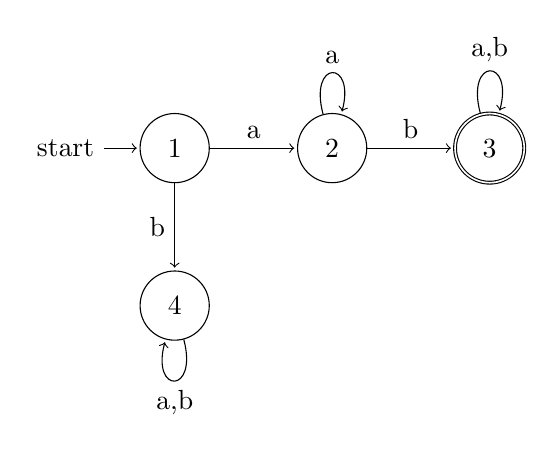
\begin{tikzpicture}[shorten >=1pt, node distance=2cm, on grid, auto] 

   \node[state, initial] (q1) {1}; 
   \node[state] (q2) [right=of q1] {2}; 
   \node[state, accepting] (q3) [right=of q2] {3}; 
   \node[state] (q4) [below=of q1] {4}; 

    \path[->]
    (q1) edge [above] node {a} (q2)
         edge [left]  node {b} (q4)
    (q2) edge [loop above] node {a} ()
         edge [above] node {b} (q3)
    (q3) edge [loop above] node {a,b} ()
    (q4) edge [loop below] node {a,b} ();
\end{tikzpicture}
\end{center}


\begin{center}
\textbf{DFA $A_2$}
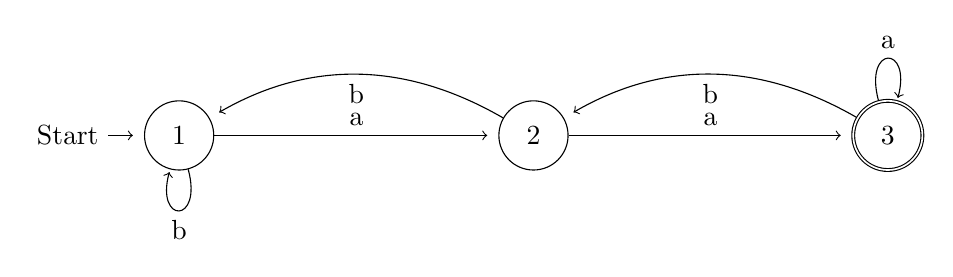
\begin{tikzpicture}[shorten >=4pt, node distance=4.5cm, on grid, auto] 

   \node[state, initial, initial text=Start] (q1) {1}; 
   \node[state] (q2) [right=of q1] {2}; 
   \node[state, accepting] (q3) [right=of q2] {3}; 

    \path[->]
    (q1) edge [above] node {a} (q2)
         edge [loop below] node {b} ()
    (q2) edge [above] node {a} (q3)
         edge [bend right=30, below] node {b} (q1)
    (q3) edge [loop above] node {a} ()
         edge [bend right=30, below] node {b} (q2);
\end{tikzpicture}
\end{center}


\textbf{Words accepted or refused by $\mathcal A_1$ and $\mathcal A_2$, respectively}
\[
\begin{array}{c|c|c}
w & \text{Accepted } A_1 & \text{Accepted } A_2 \\ \midrule
aaa & \textcolor{red}{\times} & \textcolor{green}{\checkmark} \\
aab & \textcolor{green}{\checkmark} & \textcolor{red}{\times} \\
aba & \textcolor{red}{\times} & \textcolor{red}{\times} \\
abb & \textcolor{red}{\times} & \textcolor{red}{\times} \\
baa & \textcolor{red}{\times} & \textcolor{green}{\checkmark} \\
bab & \textcolor{red}{\times} & \textcolor{red}{\times} \\
bba & \textcolor{red}{\times} & \textcolor{red}{\times} \\
bbb & \textcolor{red}{\times} & \textcolor{red}{\times} \\
\end{array}
\]
\noindent The table above summarizes the words accepted or rejected by DFA $A_1$ and DFA $A_2$. 
To implement these automata \textit{programmatically}, we define the DFA class in \texttt{dfa.py}, which allows us to process input words according to their respective state transition diagrams.

\textbf{\text{DFA Implementation in \texttt{dfa.py}}}\\
This introduction describes the design of the \texttt{dfa.py},  consisting of:
\begin{itemize}
  \item$Q$ - a finite set of states.
  \item$\Sigma$ - an input alphabet.
  \item$\delta : Q \times \Sigma \to Q$ - a transition function.
  \item$q_0 \in Q$ an initial state.
  \item$F \subseteq Q$ - a set of final accepting states.
\end{itemize}

The \texttt{DFA} class constructor takes these five elements (\texttt{Q}, \texttt{Sigma}, \texttt{delta}, \texttt{q0}, and \texttt{F}), using the method:
\begin{itemize}
  \item \texttt{run(w)}: Runs the DFA on input string \texttt{w} and determines whether or not \texttt{w} is accepted based on the state it finishes at.
\end{itemize}

\textbf{Implementation}
In the following code snippet, the \texttt{run} method processes the symbols of the input \texttt{w} sequentially, looking up the next state based on the current state and the input symbol. If an invalid transition is encountered, the method immediately returns \texttt{False}. Otherwise, if the DFA ends in a state that is a member of \texttt{F}, \texttt{True} is returned (meaning \texttt{w} is accepted); if it ends in some other state, \texttt{False} is returned.

\begin{lstlisting}
class DFA :

    # init the DFA
    def __init__(self, Q, Sigma, delta, q0, F) : 
        self.Q = Q # set of states
        self.Sigma = Sigma # set of symbols
        self.delta = delta # transition function
        self.q0 = q0 # initial state
        self.F = F # final states
   
   # print the data of the DFA
    def __repr__(self) :
        return f"DFA({self.Q},\n\t{self.Sigma},\n\t{self.delta},\n\t{self.q0},\n\t{self.F})"

    # run the DFA on the word w
    # return if the word is accepted or not
    # modify as needed
    def run(self, w) :
        # todo
        # start at initial state
        current_state = self.q0
        for symbol in w:
            if (current_state, symbol) in self.delta:
                current_state = self.delta[(current_state, symbol)]
            else:
                # invalid transition (dead state)
                return False
            # accept if in final state
        return current_state in self.F 

\end{lstlisting}

\textbf{Exercise 4: A new automaton from an old one}

Below is DFA $A_0$ which accepts exactly the words that $A$ refuses and vice versa.
\begin{center}
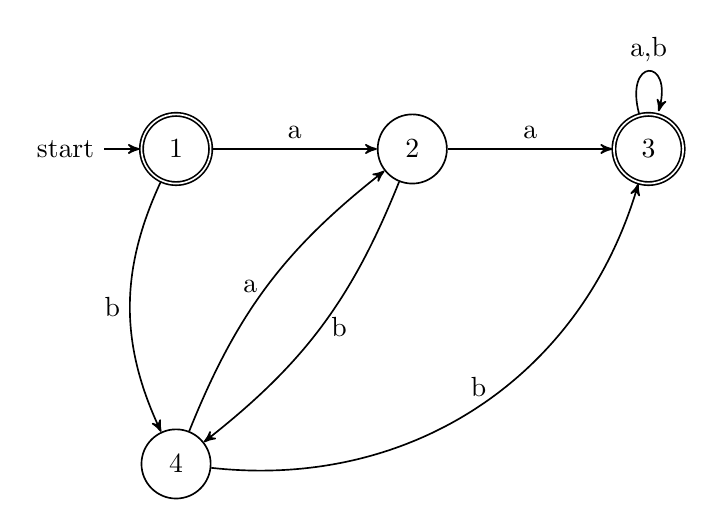
\begin{tikzpicture}[->, >=stealth', auto, semithick]
  \node[state, initial, accepting]      (q1) at (0,0)   {1};
  \node[state]                          (q2) at (3,0)   {2};
  \node[state, accepting]               (q3) at (6,0)   {3};
  \node[state]                          (q4) at (0,-4){4};
  \path
    % 1 -> 2, labeled 'a'
    (q1) edge                node[above] {a} (q2)
    % 1 -> 4, labeled 'b'
    (q1) edge[bend right=25] node[left]  {b} (q4)
    % 2 -> 3, labeled 'a'
    (q2) edge                node[above] {a} (q3)
    % 2 -> 4, labeled 'b'
    (q2) edge[bend left=15] node[right] {b} (q4)
    % 4 -> 2, labeled 'a'
    (q4) edge[bend left=15]  node[left]  {a} (q2)
    % 4 -> 3, labeled 'b'
    (q4) edge[bend right=40]  node[above] {b} (q3)
    % 3 -> 3 loop, labeled 'a,b'
    (q3) edge[loop above]    node        {a,b} ();

\end{tikzpicture}
\end{center}
In $A_0$, nodes 1 and 3 are the accepting final states, while nodes 2 and 4 are normal states.

\textbf{Exercise 2.2.4: DFAs over $\{0,1\}$}

{(a) The set of all strings ending in 00}

\noindent
\textbf{DFA Description:}
\[
\begin{aligned}
Q &= \{\,q_0,\, q_1,\, q_2\},\\
\Sigma &= \{0,1\},\\
\delta &\text{ is given by the table below},\\
q_0 &\text{ is the start state},\\
F &= \{\,q_2\}.
\end{aligned}
\]

\noindent
\textbf{Transition Table:}
\[
\begin{array}{c|cc}
  \delta & 0 & 1 \\
\hline
  q_0    & q_1 & q_0 \\
  q_1    & q_2 & q_0 \\
  q_2    & q_2 & q_0
\end{array}
\]

\noindent
\textit{Explanation:} 
\begin{itemize}
\item $q_0$ - we have not yet seen a trailing zero
\item $q_1$ - the string currently ends in exactly one zero
\item $q_2$ (accepting) - the string ends in at least two consecutive zeros
\end{itemize}

\bigskip

{(b) The set of all strings with three consecutive 0s}

\noindent
\textbf{DFA Description:}
\[
\begin{aligned}
Q &= \{\,q_0,\, q_1,\, q_2,\, q_3\},\\
\Sigma &= \{0,1\},\\
\delta &\text{ is given by the table below},\\
q_0 &\text{ is the start state},\\
F &= \{\,q_3\}.
\end{aligned}
\]

\noindent
\textbf{Transition Table:}
\[
\begin{array}{c|cc}
  \delta & 0 & 1 \\
\hline
  q_0    & q_1 & q_0 \\
  q_1    & q_2 & q_0 \\
  q_2    & q_3 & q_0 \\
  q_3    & q_3 & q_3
\end{array}
\]

\noindent
\textit{Explanation:}
\begin{itemize}
\item $q_0$ - we have seen 0 consecutive zeros so far
\item $q_1$ - we have seen exactly 1 consecutive zero
\item $q_2$ - we have seen exactly 2 consecutive zeros
\item $q_3$ (accepting) - we have seen at least 3 consecutive zeros
\end{itemize}

\bigskip

{(c) The set of all strings with \texttt{011} as a substring}

\noindent
\textbf{DFA Description:}
\[
\begin{aligned}
Q &= \{\,q_0,\, q_1,\, q_2,\, q_3\},\\
\Sigma &= \{0,1\},\\
\delta &\text{ is given by the table below},\\
q_0 &\text{ is the start state},\\
F &= \{\,q_3\}.
\end{aligned}
\]

\noindent
\textbf{Transition Table:}
\[
\begin{array}{c|cc}
  \delta & 0 & 1 \\
\hline
  q_0    & q_1 & q_0 \\
  q_1    & q_1 & q_2 \\
  q_2    & q_1 & q_3 \\
  q_3    & q_3 & q_3
\end{array}
\]

\noindent
\textit{Explanation:}
\begin{itemize}
\item $q_0$ - no partial match yet
\item $q_1$ - we matched a single \texttt{0}
\item $q_2$ - we matched \texttt{01}
\item $q_3$ (accepting) - we found \texttt{011} somewhere in the string
\end{itemize}
\bigskip

\subsection{\textbf{Week 4}}\\
\textbf{Lecture Summary}\\
%Summarize when I get the chance
We explore the concept of \emph{product automata} and how they can be used to model operations on languages accepted by two deterministic finite automata (DFAs). In particular, we discuss how to construct an automaton that accepts the intersection (or union) of the languages recognized by two given automata.

\textbf{Homework 3}

\textbf{Problem 1: Extended transition function}\\
Consider two DFAs:
\[
\mathcal{A}^{(1)} = \big(Q^{(1)}, \Sigma, \delta^{(1)}, q_0^{(1)}, F^{(1)}\big) \quad \text{and} \quad \mathcal{A}^{(2)} = \big(Q^{(2)}, \Sigma, \delta^{(2)}, q_0^{(2)}, F^{(2)}\big),
\] 
\\over the alphabet $\Sigma = \{a, b\}$.
\begin{center}
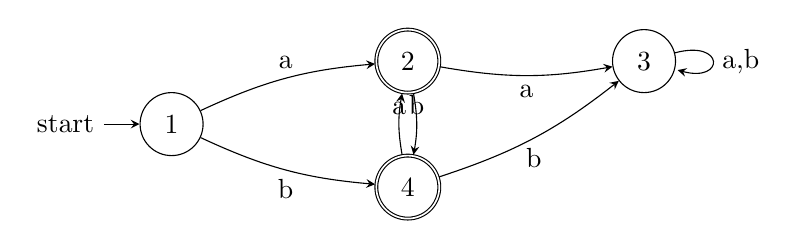
\begin{tikzpicture}[>=stealth,node distance=2.5cm,on grid,auto]
\tikzstyle{state}=[circle,draw,minimum size=8mm,inner sep=0pt]

  %--- nodes ---
  \node[state, initial] (1) {1};
  \node[state, accepting] (2) [right=3cm of 1, yshift=0.8cm] {2};
  \node[state, accepting] (4) [right=3cm of 1, yshift=-0.8cm] {4};
  \node[state] (3) [right=3cm of 2] {3};

  %--- transitions ---
  \path[->]
    (1) edge[bend left=10] node[above] {a} (2)
    (1) edge[bend right=10] node[below] {b} (4)

    (2) edge[bend left=10] node[above] {b} (4)
    (2) edge[bend right=10] node[below] {a} (3)

    (4) edge[bend left=10] node[above] {a} (2)
    (4) edge[bend right=10] node[below] {b} (3)

    (3) edge[loop right] node {a,b} (3);
\end{tikzpicture}
\end{center}

\noindent
\textit{Diagram for \(A^{(1)}\):}
\begin{itemize}
  \item State 1 is the initial state (arrow from the left).
  \item From state 1: reading `\(a\)' goes to 2; reading `\(b\)' goes to 4.
  \item From state 2: reading `\(a\)' goes to 3; reading `\(b\)' goes to 4.
  \item From state 4: reading `\(a\)' goes to 2; reading `\(b\)' goes to 3.
  \item From state 3: reading either `\(a\)' or `\(b\)' loops on 3.
  \item States 2 and 4 are accepting, while state 3 is a non-accepting sink.
\end{itemize}

\bigskip

\begin{center}
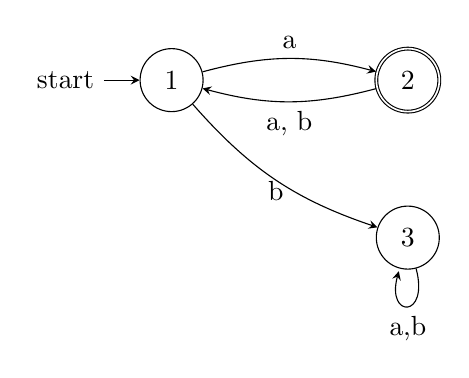
\begin{tikzpicture}[>=stealth,node distance=2.5cm,on grid,auto]
\tikzstyle{state}=[circle,draw,minimum size=8mm,inner sep=0pt]

%--- nodes ---
\node[state, initial] (1) {1};
\node[state, accepting] (2) [right=3cm of 1] {2};
\node[state] (3) [below=2cm of 2] {3};

%--- initial arrow ---
\path[->] 
  node[above left=0.5cm of 1]{}
  (1);

%--- transitions ---
\path[->]
  (1) edge[bend left=15] node[above] {a} (2)
  (1) edge[bend right=15] node[left,pos=0.6] {b} (3)
  (2) edge[bend left=15] node[below] {a, b} (1)
  (3) edge[loop below] node {a,b} (3);

\end{tikzpicture}
\end{center}

\noindent
\textit{Diagram for \(A^{(2)}\):}
\begin{itemize}
  \item State 1 is the initial state (arrow from the left).
  \item From state 1: reading `\(a\)' goes to 2; reading `\(b\)' goes to 3.
  \item From state 2: reading `\(a\)' or `\(b\)' goes back to 1.
  \item State 3 loops on both `\(a\)' and `\(b\)'.
  \item State 2 is the only accepting state.
\end{itemize}

\textbf{a. Descriptions of Accepted Languages}

\begin{itemize}
    \item \textbf{$\mathcal{A}^{(1)}$:} Accepts non-empty words in which no two consecutive letters are the same.
    \item \textbf{$\mathcal{A}^{(2)}$:} Accepts words of odd length where every letter at an odd position of $w$ is the letter $a$.
\end{itemize}
Hence,
\[
L\bigl(A^{(2)}\bigr)
=\bigl\{\,w \in \{a,b\}^* \,\mid\, |w|\text{ is odd and the odd-indexed letters are all }a\bigr\}.
\]

\bigskip

\textbf{b. Computation: $\widehat{\delta}^{(1)}\bigl(1,\texttt{abaa}\bigr)$}

The automaton $A^{(1)}$ has states $\{1,2,3,4\}$, where:
\begin{itemize}
    \item State 1 is the initial state (non-final).
    \item State 2 indicates the last letter read was $a$ (no violation).
    \item State 4 indicates the last letter read was $b$ (no violation).
    \item State 3 is the ``sink'' or ``trap'' state (once a violation occurs, e.g.\ two consecutive letters the same).
\end{itemize}
We compute step-by-step for the input \(\texttt{abaa}\):
\[
\widehat{\delta}^{(1)}(1,\texttt{abaa}):
\]
\begin{enumerate}
    \item Start in state $1$, input = \texttt{abaa}.
    \item Read `a': $\delta^{(1)}(1,a) = 2$. Remaining input = \texttt{baa}.
    \item Now in state $2$, read `b': $\delta^{(1)}(2,b) = 4$. Remaining input = \texttt{aa}.
    \item Now in state $4$, read `a': $\delta^{(1)}(4,a) = 2$. Remaining input = \texttt{a}.
    \item Now in state $2$, read `a': $\delta^{(1)}(2,a) = 3$. Remaining input is empty.
\end{enumerate}
Therefore,
\[
\widehat{\delta}^{(1)}(1,\texttt{abaa}) \;=\; 3.
\]
Since state $3$ is the non-accepting sink, the string \texttt{abaa} is not accepted by $A^{(1)}$.

\bigskip

\textbf{b. Computation: $\widehat{\delta}^{(2)}\bigl(1,\texttt{abba}\bigr)$}

Automaton $A^{(2)}$ can be thought of as having states:
\begin{itemize}
    \item State 1: an even number of letters read so far (initial, non-final).
    \item State 2: an odd number of letters read so far, with ``odd positions must be $a$'' still satisfied (accepting).
    \item State 3: dead/trap state (if the condition on odd positions is violated).
\end{itemize}
We compute for \(\texttt{abba}\) (positions are 1,2,3,4):
\[
\widehat{\delta}^{(2)}(1,\texttt{abba}):
\]
\begin{enumerate}
    \item Start in state $1$, input = \texttt{abba}.
    \item Read `a' (position 1): $\delta^{(2)}(1,a) = 2$. Remaining input = \texttt{bba}.
    \item Now in state $2$, read `b' (position 2): $\delta^{(2)}(2,b) = 1$. Remaining input = \texttt{ba}.
    \item Now in state $1$, read `b' (position 3): $\delta^{(2)}(1,b) = 3$. Remaining input = \texttt{a}.
    \item Now in state $3$, read `a': $\delta^{(2)}(3,a) = 3$. Remaining input is empty.
\end{enumerate}
Hence,
\[
\widehat{\delta}^{(2)}(1,\texttt{abba}) = 3,
\]
and state $3$ is non-accepting. Therefore, \texttt{abba} is not accepted by $A^{(2)}$.

\bigskip

\textbf{Problem 2: Product automata}

We now define a \emph{product automaton} $A$ from $A^{(1)}$ and $A^{(2)}$ in order to recognize 
\[
L\bigl(A^{(1)}\bigr) \;\cap\; L\bigl(A^{(2)}\bigr).
\]

\subsubsection*{a. Construct the intersection automaton $A$}

\noindent \textbf{States.} The state set of $A$ is the Cartesian product
\[
Q \;=\; Q^{(1)} \;\times\; Q^{(2)}.
\]
If $Q^{(1)} = \{1,2,3,4\}$ and $Q^{(2)} = \{1,2,3\}$, then
\[
Q = \{(1,1),(1,2),(1,3),(2,1),(2,2),(2,3),(3,1),(3,2),(3,3),(4,1),(4,2),(4,3)\}.
\]

\noindent \textbf{Initial state.} $(1,1)$, since $1$ is the initial state of $A^{(1)}$ and $1$ is the initial state of $A^{(2)}$.

\noindent \textbf{Transition function.} For $(p,q)\in Q$ and $x \in \{a,b\}$,
\[
\delta\bigl((p,q),x\bigr) \;=\; \bigl(\delta^{(1)}(p,x),\;\delta^{(2)}(q,x)\bigr).
\]

\noindent \textbf{Final states (for intersection).} A pair $(p,q)$ is final if $p \in F^{(1)}$ and $q \in F^{(2)}$. 
- For $A^{(1)}$, we have $F^{(1)} = \{2,4\}$ (all non-empty strings with no two consecutive letters the same).  
- For $A^{(2)}$, we have $F^{(2)} = \{2\}$ (odd-length strings with \(a\) in every odd position).

Thus
\[
F \;=\; \{(p,q) \mid p \in \{2,4\},\, q = 2\}.
\]

\paragraph{Diagram of product automaton $A$}showing all transitions. For brevity, not every state is drawn if some are unreachable.

\begin{center}
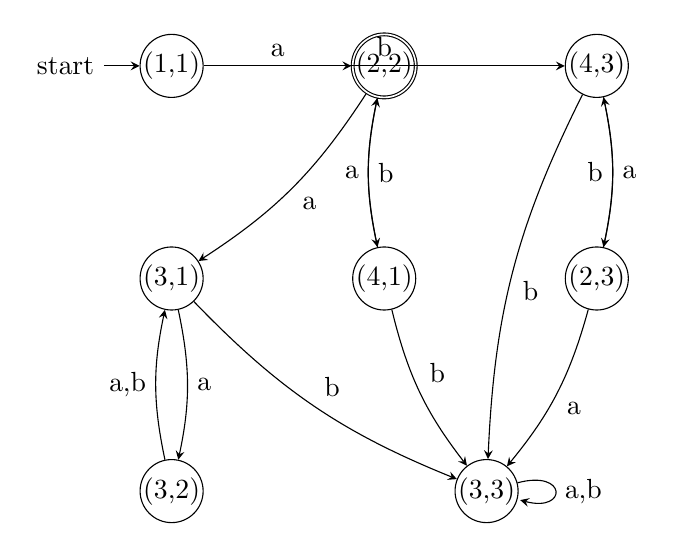
\begin{tikzpicture}[>=stealth,node distance=2.7cm,on grid,auto]
\tikzstyle{state}=[circle,draw,minimum size=8mm,inner sep=0pt]

%-- Nodes that are reachable only  --
\node[state, initial] (11) {(1,1)};
\node[state, accepting] (22) [right of=11] {(2,2)};
\node[state] (43) [right of=22] {(4,3)};
\node[state] (31) [below of=11] {(3,1)};
\node[state] (41) [below of=22] {(4,1)};
\node[state] (23) [below of=43] {(2,3)};
\node[state] (32) [below of=31] {(3,2)};
\node[state] (33) [below of=41, xshift=1.3cm] {(3,3)};

%-- Transitions --
\path[->]
  % (1,1)
  (11) edge node {a} (22)
  (11) edge node {b} (43)

  % (2,2)
  (22) edge[bend left=12] node {a} (31)
  (22) edge[bend right=12] node {b} (41)

  % (4,3)
  (43) edge[bend left=12] node {a} (23)
  (43) edge[bend right=12] node {b} (33)

  % (3,1)
  (31) edge[bend left=12] node {a} (32)
  (31) edge[bend right=12] node {b} (33)

  % (4,1)
  (41) edge[bend left=12] node {a} (22)
  (41) edge[bend right=12] node {b} (33)

  % (2,3)
  (23) edge[bend left=12] node {a} (33)
  (23) edge[bend right=12] node {b} (43)

  % (3,2)
  (32) edge[bend left=12] node {a,b} (31)

  % (3,3)
  (33) edge[loop right] node {a,b} (33);

\end{tikzpicture}
\end{center}

\subsubsection*{b. Why $L(A) = L\bigl(A^{(1)}\bigr)\,\cap\,L\bigl(A^{(2)}\bigr)$}

A string $w$ is accepted by $A$ precisely if:
\begin{itemize}
    \item Following the transitions of $A$ on $w$ leads from $(1,1)$ to a final state $(p,q)$.
    \item This happens exactly when $p$ is a final state of $A^{(1)}$ \emph{and} $q$ is a final state of $A^{(2)}$.
\end{itemize}
Thus $w$ is accepted by both $A^{(1)}$ and $A^{(2)}$. Hence $L(A) = L(A^{(1)}) \cap L(A^{(2)})$.

\subsubsection*{c. Constructing $A'$ for the Union}

To get $L(A') = L\bigl(A^{(1)}\bigr) \cup L\bigl(A^{(2)}\bigr)$, we keep the same product structure but change the final states. A product state $(p,q)$ is final if \emph{either} $p \in F^{(1)}$ \emph{or} $q \in F^{(2)}$. Formally:
\[
F' \;=\; \bigl(F^{(1)} \times Q^{(2)}\bigr) \;\cup\;\bigl(Q^{(1)} \times F^{(2)}\bigr).
\]
This ensures that a string is accepted by $A'$ if it is accepted by $A^{(1)}$ \emph{or} $A^{(2)}$.

\bigskip

\noindent \textbf{Summary of Key Points:}
\begin{itemize}
    \item For $A^{(1)}$, the accepting states are $\{2,4\}$; consecutive letters must differ and the string must be non-empty.
    \item For $A^{(2)}$, the accepting state is $\{2\}$; the string must have odd length and $a$ in every odd position.
    \item Extended transitions showed that $\widehat{\delta}^{(1)}(1,\texttt{abaa}) = 3$ (not accepted) and $\widehat{\delta}^{(2)}(1,\texttt{abba}) = 3$ (not accepted).
    \item The product automaton for intersection has final states $F^{(1)} \times F^{(2)} = \{(2,2), (4,2)\}$, while for union we use $F' = (F^{(1)} \times Q^{(2)}) \;\cup\; (Q^{(1)} \times F^{(2)})$.
\end{itemize}
\bigskip\bigskip\bigskip\bigskip\bigskip\bigskip\bigskip\bigskip\bigskip\bigskip\bigskip\bigskip

\textbf{Exercise 2.2.7: Induction Proof}

\noindent
\textbf{Statement:} Let $A$ be a DFA, and let $q$ be a particular state of $A$ such that
\[
\delta(q,a) \;=\; q
\quad
\text{for all input symbols } a.
\]
Show by induction on the length of the input that for all input strings $w$, we have
\[
\widehat{\delta}(q,w) \;=\; q.
\]

\bigskip

\noindent
\textbf{Proof (by induction on the length of $w$):}

\paragraph{Base Case ($|w| = 0$):}
If $w$ is the empty string $\epsilon$, then by definition of the extended transition function,
\[
\widehat{\delta}(q,\epsilon) \;=\; q.
\]
Hence the statement holds for $|w| = 0$.

\paragraph{Inductive Step:}
Assume that for all strings $x$ of length $n$, we have
\[
\widehat{\delta}(q,x) \;=\; q.
\]
We need to prove the statement for any string $w$ of length $n+1$. Let $w$ be such a string. We can write $w$ as
\[
w \;=\; x\,a,
\]
where $x$ is a string of length $n$, and $a$ is a single input symbol. Then,
\[
\widehat{\delta}(q,w)
\;=\;
\widehat{\delta}(q,\,x\,a)
\;=\;
\delta\bigl(\widehat{\delta}(q,x),\,a\bigr).
\]
By the inductive hypothesis, $\widehat{\delta}(q,x) = q$. Therefore,
\[
\widehat{\delta}(q,w)
\;=\;
\delta(q,a).
\]
But we are given that $\delta(q,a) = q$ for all symbols $a$. Hence,
\[
\widehat{\delta}(q,w)
\;=\;
q.
\]
This completes the inductive step.

\paragraph{Conclusion:}
By the principle of mathematical induction, for all strings $w$, we have
\[
\widehat{\delta}(q,w) = q.
\]
Thus, if a state $q$ transitions to itself on every symbol, it remains $q$ under any input string.
\paragraph{ITALC 2.3 Question:}
In the subset construction for converting an NFA to a DFA, often there is an exponential blow-up in the number of states. Can you propose a scenario for which this blow-up actually happens, and whether there are any strategies or special cases that might mitigate this worst-case behavior?


\subsection{\textbf{Week 5}}\\
\textbf{Lecture Summary}\\
%Summarize when I get the chance
TBD

\textbf{Homework 4}\\
\textbf{Problem 1: NFA Interpretation}
We can consider $A$ as an NFA because each transition goes to a 
single-element set (instead of exactly one state). Hence, $A$ 
can be viewed as a valid NFA.

\[
A' = \bigl(Q', \Sigma, \delta', q'_0, F'\bigr),
\]
where
\[
Q' = Q, 
\quad
q'_0 = q_0, 
\quad
F' = F,
\quad
\delta'(q,a) = \{\delta(q,a)\}.
\]

\textbf{2. Why it works.}

Each string accepted by $A$ has the exact same single path of states 
in $A'$, because $\delta'$ uses the same transitions as $\delta$, 
but returns them as singleton sets. 
Thus, every string accepted by $A'$ follows that same single path of 
states in $A$. Consequently,
\[
L(A') \;=\; L(A).
\]

\textbf{Problem 2:}
The NFA $A$ has four states $q_0, q_1, q_2, q_3$, with $q_0$ as the 
start state and $q_3$ as the (only) accepting state. The transitions are:
\[
\delta(q_0,0) = \{q_0\}, \quad
\delta(q_0,1) = \{q_1\},
\]
\[
\delta(q_1,0) = \{q_2\}, \quad
\delta(q_1,1) = \emptyset,
\]
\[
\delta(q_2,0) = \{q_3\}, \quad
\delta(q_2,1) = \{q_0\},
\]
\[
\delta(q_3,0) = \{q_3\}, \quad
\delta(q_3,1) = \{q_3\}.
\]

By analyzing all possible paths, we can determine that the language accepted by $A$ is:
\[
L(A) = \{w \in \{0,1\}^* \mid w \text{ contains the substring } 100 \text{ or } w \text{ ends with } 10\}
\]

\textbf{2. Specify $A$ in the form $(Q,\Sigma,\delta,q_0,F)$}

\[
Q = \{q_0,\, q_1,\, q_2,\, q_3\}, \quad
\Sigma = \{0,1\}, \quad
q_0 \text{ is the start state}, \quad
F = \{q_3\}.
\]
The transition function $\delta$ is as above.

\textbf{3. Compute $\hat{\delta}\bigl(q_0,\,10110\bigr)$ step by step}

We track the set of possible states after each input symbol:

\begin{enumerate}
\item Start: $\{q_0\}$.
\item Read `1`: $\delta(q_0,1) = \{q_1\}$, so now in $\{q_1\}$.
\item Read `0`: $\delta(q_1,0) = \{q_2\}$, so now in $\{q_2\}$.
\item Read `1`: $\delta(q_2,1) = \{q_0\}$, so now in $\{q_0\}$.
\item Read `1`: $\delta(q_0,1) = \{q_1\}$, so now in $\{q_1\}$.
\item Read `0`: $\delta(q_1,0) = \{q_2\}$, so now in $\{q_2\}$.
\end{enumerate}

Thus,
\[
\hat{\delta}(q_0,\,10110) \;=\; \{q_2\}.
\]
Since $q_2 \notin F$, the string $10110$ is not accepted.

\textbf{4. Find all paths in $A$ for $v = 1100$ and $w = 1010$}

\paragraph{For $v = 1100$:}
\[
q_0 \xrightarrow{\,1\,} q_1 \xrightarrow{\,1\,} \emptyset
\]
The computation halts at the second symbol since $\delta(q_1,1) = \emptyset$. No path exists for the entire string, so it's not accepted.

\paragraph{For $w = 1010$:}
\[
q_0 \xrightarrow{\,1\,} q_1 
\xrightarrow{\,0\,} q_2 
\xrightarrow{\,1\,} q_0 
\xrightarrow{\,0\,} q_0
\]
We end in $q_0$, which is not an accepting state, so $1010$ is not accepted.

\textbf{5. Construct the determinization $A^D$ (power-set construction)}

We list the reachable subsets of $\{q_0, q_1, q_2, q_3\}$:

\begin{itemize}
\item \textbf{Start state}: $\{q_0\}$. 
  \begin{itemize}
  \item On $0$: $\{q_0\}$.
  \item On $1$: $\{q_1\}$.
  \end{itemize}
\item \textbf{State} $\{q_1\}$.
  \begin{itemize}
  \item On $0$: $\{q_2\}$.
  \item On $1$: $\emptyset$.
  \end{itemize}
\item \textbf{State} $\{q_2\}$.
  \begin{itemize}
  \item On $0$: $\{q_3\}$.
  \item On $1$: $\{q_0\}$.
  \end{itemize}
\item \textbf{State} $\{q_3\}$.
  \begin{itemize}
  \item On $0$: $\{q_3\}$.
  \item On $1$: $\{q_3\}$.
  \end{itemize}
\item \textbf{Dead state} $\emptyset$.
  \begin{itemize}
  \item On $0$: $\emptyset$.
  \item On $1$: $\emptyset$.
  \end{itemize}
\end{itemize}

The start state in the DFA is $\{q_0\}$, and the accepting states are 
all subsets containing $q_3$, namely $\{q_3\}$.

\textbf{6. Verify $L(A) = L(A^D)$. Is there a smaller DFA?}

By the standard subset construction, we have $L(A^D) = L(A)$. 
Since $L(A)$ is the set of strings that either contain the substring $100$ or end with $10$, 
one might suspect a smaller DFA could exist. However, standard DFA 
minimization shows that all the reachable states in $A^D$ are pairwise 
inequivalent, so no merges are possible without altering the language. 
Hence, the $5$-state DFA (including the dead state $\emptyset$) is already minimal.

\textbf{Question:} Can you describe a practical scenario where combining the two (i.e first designing an NFA and then converting or integrating it into a DFA) provides benefits that neither approach alone can normally offer?


\subsection{\textbf{Week 6}}\\
\textbf{Lecture Summary}\\
%Summarize when I get the chance
TBD

\textbf{Homework 5}\\
\textbf{Exercise 3.2.1: Analysis of a DFA and Regular Expressions}

Consider the DFA with the following transition table:
\begin{center}
\begin{tabular}{c|cc}
 & 0 & 1 \\ \hline
$\to q_0$ & $q_0$ & $q_1$ \\
$q_1$ & $q_2$ & $q_3$ \\
$q_2$ & $q_2$ & $q_3$ \\
$*q_3$ & $q_2$ & $q_3$ \\
\end{tabular}
\end{center}

\textbf{a. Regular expression $R^0_0$}

$R^0_0$ represents paths from $q_0$ to $q_0$ using only states $\{q_0\}$ as intermediate states.
$R^0_0 = 0^*$

\textbf{b. Regular expressions $R^1_{ij}$}

Adding $q_1$ as an intermediate state:
\begin{align*}
R^1_{00} &= R^0_{00} + R^0_{01}(R^0_{11})^*R^0_{10} = 0^* + (0^*1)(0 \cdot 0^*)^* \cdot \emptyset = 0^* \\
R^1_{01} &= R^0_{01} + R^0_{01}(R^0_{11})^*R^0_{11} = 0^*1 + (0^*1)(0 \cdot 0^*)^* \cdot 0 = 0^*1 \\
R^1_{02} &= R^0_{02} + R^0_{01}(R^0_{11})^*R^0_{12} = \emptyset + (0^*1)(0 \cdot 0^*)^* \cdot 0 = 0^*10 \\
R^1_{03} &= R^0_{03} + R^0_{01}(R^0_{11})^*R^0_{13} = \emptyset + (0^*1)(0 \cdot 0^*)^* \cdot 1 = 0^*11 \\
\end{align*}

\textbf{c. Regular expressions $R^2_{ij}$}

Adding $q_2$ as an intermediate state:
\begin{align*}
R^2_{03} &= R^1_{03} + R^1_{02}(R^1_{22})^*R^1_{23} = 0^*11 + (0^*10)(0^*)^*1 = 0^*11 + 0^*100^*1 \\
\end{align*}

\textbf{d. Regular expression for the language}

The language accepted by this DFA consists of all strings that lead from the start state $q_0$ to the accepting state $q_3$. This is represented by $R^3_{03}$.

After completing all steps of the state-elimination method:
$R^3_{03} = 0^*1(1+00^*1)$

This can be simplified to:
$R = 0^*1(1+00^*1)$

\textbf{e. Simplified transition diagram}

We can construct a simplified transition diagram by eliminating state $q_0$ and using the computed regular expression to describe the language directly. The resulting automaton has $q_0$ as the start state, with a transition on $0^*1$ to $q_1$, and then transitions as in the original diagram for the remaining states, with $q_3$ as the accepting state.

\textbf{Exercise 3.2.2: Analysis of Another DFA}

Consider the NFA with the following transition table:
\begin{center}
\begin{tabular}{c|cc}
 & a & b \\ \hline
$\to q_0$ & $\{q_0,q_1\}$ & $\{q_0\}$ \\
$q_1$ & $\emptyset$ & $\{q_2\}$ \\
$q_2$ & $\{q_3\}$ & $\emptyset$ \\
$*q_3$ & $\emptyset$ & $\emptyset$ \\
\end{tabular}
\end{center}

\textbf{a. Regular expressions for each state}

Using the state-elimination method, we first compute basic paths:
\begin{align*}
R^0_{00} &= a^* \\
R^0_{01} &= a^*a = a^+ \\
R^0_{02} &= a^+b \\
R^0_{03} &= a^+ba \\
\end{align*}

\textbf{b. Regular expressions with elimination}

Continuing the state-elimination method, we eliminate states $q_1$ and $q_2$ in sequence:
\begin{align*}
R^2_{03} &= a^+ba + \emptyset = a^+ba \\
\end{align*}

\textbf{c. Final regular expression}

The language accepted by this NFA can be described by the regular expression:
$R = a^+ba$

This represents strings that start with one or more 'a's, followed by a 'b', followed by an 'a'.

\textbf{d. Constructing the determinized DFA}

Following the subset construction for this NFA, we get the following DFA:
\begin{itemize}
    \item Start state: $S_0 = \{q_0\}$
    \item On input 'a': $\delta'(S_0,a) = \{q_0,q_1\} = S_1$
    \item On input 'b': $\delta'(S_0,b) = \{q_0\} = S_0$
    \item From $S_1 = \{q_0,q_1\}$:
      \begin{itemize}
        \item On input 'a': $\delta'(S_1,a) = \{q_0,q_1\} = S_1$
        \item On input 'b': $\delta'(S_1,b) = \{q_0,q_2\} = S_2$
      \end{itemize}
    \item From $S_2 = \{q_0,q_2\}$:
      \begin{itemize}
        \item On input 'a': $\delta'(S_2,a) = \{q_0,q_1,q_3\} = S_3$
        \item On input 'b': $\delta'(S_2,b) = \{q_0\} = S_0$
      \end{itemize}
    \item From $S_3 = \{q_0,q_1,q_3\}$ (accepting state):
      \begin{itemize}
        \item On input 'a': $\delta'(S_3,a) = \{q_0,q_1\} = S_1$
        \item On input 'b': $\delta'(S_3,b) = \{q_0,q_2\} = S_2$
      \end{itemize}
\end{itemize}

\textbf{Exercise 4.4.1: DFA Minimization via Distinguishability}

Consider the DFA with states $\{A, B, C, D, E, F, G\}$, where the start state is $A$ and the only final state is $D$. The transition function is given in the table:

\begin{center}
\begin{tabular}{c|cc}
\textbf{State} & \textbf{0} & \textbf{1} \\ \hline
$A$ & $B$ & $F$ \\
$B$ & $G$ & $C$ \\
$C$ & $A$ & $C$ \\
$*D$ & $D$ & $E$ \\
$E$ & $D$ & $C$ \\
$F$ & $F$ & $G$ \\
$G$ & $G$ & $E$ \\
\end{tabular}
\end{center}

\textbf{a. Table of Distinguishability}

We first mark pairs where one state is final and the other is not: $(A,D)$, $(B,D)$, $(C,D)$, $(D,E)$, $(D,F)$, and $(D,G)$.

Next, we examine all unmarked pairs to see if their transitions lead to marked pairs:
\begin{itemize}
    \item For pair $(A,B)$: on input 0, transitions to $(B,G)$; on input 1, to $(F,C)$.
    \item For pair $(A,C)$: on input 0, transitions to $(B,A)$; on input 1, to $(F,C)$.
    \item And so on...
\end{itemize}

After iteratively marking pairs until no more can be marked, we find that the following pairs remain unmarked:
$(E,G)$ and $(F,G)$

This means states $E$ and $G$ are equivalent, and states $F$ and $G$ are equivalent. By transitivity, all three states $E$, $F$, and $G$ are equivalent.

\textbf{b. The Minimum-State Equivalent DFA}

By merging the equivalent states $E$, $F$, and $G$ into a single state $[EFG]$, the minimized DFA has the following states:
$\{A, B, C, D, [EFG]\}$

The transition function for the minimized DFA is:
\begin{itemize}
    \item $A$: $0 \to B$, $1 \to [EFG]$
    \item $B$: $0 \to [EFG]$, $1 \to C$
    \item $C$: $0 \to A$, $1 \to C$
    \item $D$: $0 \to D$, $1 \to [EFG]$
    \item $[EFG]$: $0 \to [EFG]$, $1 \to [EFG]$
\end{itemize}

The start state is $A$ and the only accepting state is $D$. The minimized DFA has 5 states.

\textbf{Exercise 4.4.2: Minimization of Another DFA}

Consider the DFA with states $\{A, B, C, D, E, F, G, H, I\}$, with $A$ as the start state and $C$ and $I$ as final states, with transitions as shown in the table:

\begin{center}
\begin{tabular}{c|cc}
\textbf{State} & \textbf{0} & \textbf{1} \\ \hline
$A$ & $B$ & $F$ \\
$B$ & $C$ & $G$ \\
$*C$ & $D$ & $H$ \\
$D$ & $E$ & $A$ \\
$E$ & $I$ & $B$ \\
$F$ & $G$ & $C$ \\
$G$ & $H$ & $D$ \\
$H$ & $A$ & $E$ \\
$*I$ & $F$ & $I$ \\
\end{tabular}
\end{center}

\textbf{a. Table of Distinguishability}

We begin by marking all pairs where exactly one state is final: 
$(A,C)$, $(A,I)$, $(B,C)$, $(B,I)$, $(C,D)$, $(C,E)$, $(C,F)$, $(C,G)$, $(C,H)$, $(D,I)$, $(E,I)$, $(F,I)$, $(G,I)$, and $(H,I)$.

Next, we iteratively mark additional pairs if their transitions lead to marked pairs. After completing this process, we find that the following pairs remain unmarked:
$(A,H)$, $(B,G)$, $(D,F)$, and $(E,C)$

This means that states $A$ and $H$ are equivalent, states $B$ and $G$ are equivalent, states $D$ and $F$ are equivalent, and states $E$ and $C$ are equivalent.

\textbf{b. The Minimum-State DFA}

By merging equivalent states, the minimized DFA has these states:
$\{[AH], [BG], [CF], [DE], I\}$

The transition function for the minimized DFA is:
\begin{itemize}
    \item $[AH]$: $0 \to [BG]$, $1 \to [CF]$
    \item $[BG]$: $0 \to [CF]$, $1 \to [DE]$
    \item $[CF]$: $0 \to [DE]$, $1 \to [AH]$
    \item $[DE]$: $0 \to I$, $1 \to [BG]$
    \item $I$: $0 \to [DE]$, $1 \to I$
\end{itemize}

The start state is $[AH]$ and the accepting states are $[CF]$ and $I$. The minimized DFA has 5 states.

\textbf{ITALC Question:}
In practice, is it always worth fully minimizing a DFA when implementing features like pattern matching or lexical analysis? What are the trade-offs between the computational cost of minimization and the runtime efficiency gained?

\subsection{\textbf{Week 7}}\\
\textbf{Lecture Summary}\\
TBD

\textbf{Homework 6}\\
\textbf{Exercise A:}\\
\begin{enumerate}
  \item \textbf{Input language:} \(L = \{\,1\,0^n : n\in\mathbb{N}\}\). on input \(1\,0^n\) the TM must output \(1\,0^{n+1}\).

        \[
          M_1 = (Q,\Sigma,\Gamma,\delta,q_0,B,F)
        \]
        \(Q=\{q_0,q_1,q_{\mathrm{accept}},q_{\mathrm{reject}}\},\;
          \Sigma=\{0,1\},\;
          \Gamma=\{0,1,B\},\;
          F=\{q_{\mathrm{accept}}\}\).

        \[
        \begin{array}{r|ccc}
                 & 0                  & 1                         & B \\ \hline
        q_0      & (q_{\mathrm{reject}},0,R) & (q_1,1,R)                 &  - \\
        q_1      & (q_1,0,R)          & (q_{\mathrm{reject}},1,R) & (q_{\mathrm{accept}},0,R)\\
        q_{\mathrm{accept}} & \multicolumn{3}{c}{\text{halt+accept}}\\
        q_{\mathrm{reject}} & \multicolumn{3}{c}{\text{halt+reject}}\\
        \end{array}
        \]

  \item \textbf{Input language:} \(L = \{\,1\,0^n : n\in\mathbb{N}\}\). on input \(1\,0^n\) the TM must leave just the leading \(1\).

        \[
          M_2 = (Q,\Sigma,\Gamma,\delta,q_0,B,F)
        \]
        \(Q=\{q_0,q_1,q_{\mathrm{accept}},q_{\mathrm{reject}}\}\).

        \[
        \begin{array}{r|ccc}
                 & 0                  & 1                         & B \\ \hline
        q_0      & (q_{\mathrm{reject}},0,R) & (q_1,1,R)                 &  - \\
        q_1      & (q_1,B,R)          & (q_{\mathrm{reject}},1,R) & (q_{\mathrm{accept}},B,R)\\
        q_{\mathrm{accept}} & \multicolumn{3}{c}{\text{halt+accept}}\\
        q_{\mathrm{reject}} & \multicolumn{3}{c}{\text{halt+reject}}\\
        \end{array}
        \]

  \item \textbf{Input language:} all binary strings. the TM outputs the bitwise complement (swap \(0\leftrightarrow1\)).

        \[
          M_3 = (Q,\Sigma,\Gamma,\delta,q_0,B,F),\;
          Q=\{q_0,q_{\mathrm{accept}}\}
        \]

        \[
        \begin{array}{r|ccc}
                 & 0          & 1          & B \\ \hline
        q_0      & (q_0,1,R)  & (q_0,0,R)  & (q_{\mathrm{accept}},B,R)\\
        q_{\mathrm{accept}} & \multicolumn{3}{c}{\text{halt+accept}}\\
        \end{array}
        \]
\end{enumerate}

    \textbf{Question: }If we encode the step bound \(k\) in unary (\(1^{k}\)) instead of binary, does the language  
        \(L_{3} = \{\langle M,w,k\rangle \mid M \text{ halts on } w \text{ in } \le k \text{ steps}\}\)  
        remain decidable, or does the change in encoding alter its classification?  

\subsection{\textbf{Week 8}}\\
\textbf{Lecture Summary}\\
TBD

\textbf{Homework 7}\\
\textbf{Exercise 1: Decidability}\\
Classify each language as \emph{decidable}, \emph{recursively enumerable (r.e.)}, or \emph{co‑r.e.}. 

\begin{enumerate}
  \item \(L_1 = \{\,M \mid M \text{ halts on itself}\}\)  
        \begin{itemize}
          \item \textbf{r.e.\ but not decidable}; not co‑r.e.  
          \item Argument: Simulate \(M\) on its own description; accept if it halts (semi‑decider).  
                Decidable would imply a solution to the halting problem.
        \end{itemize}

  \item \(L_2 = \{\,\langle M,w\rangle \mid M \text{ halts on } w\}\)  
        \begin{itemize}
          \item \textbf{r.e.\ but not decidable}; not co‑r.e.  
          \item Classic halting problem.
        \end{itemize}

  \item \(L_3 = \{\,\langle M,w,k\rangle \mid M \text{ halts on } w \text{ in } \le k \text{ steps}\}\)  
        \begin{itemize}
          \item \textbf{Decidable} (thus both r.e.\ and co‑r.e.).  
          \item Simulate exactly \(k\) steps, accept if halts; otherwise reject.
        \end{itemize}

        
\end{enumerate}

\bigskip
\textbf{Exercise 2: Closure Properties}\\
For each statement, indicate True/False and give justification.

\begin{enumerate}
  \item \(\;L_1, L_2\) decidable \(\Rightarrow L_1 \cup L_2\) decidable. \textbf{True}.  
        Run both deciders; accept if either accepts.

  \item \(L\) decidable \(\Rightarrow \overline{L}\) decidable. \textbf{True}.  
        Flip the accept/reject outcome.

  \item \(L\) decidable \(\Rightarrow L^{*}\) decidable. \textbf{True}.  
        Enumerate all segmentations; dynamic‑programming decider halts.

  \item \(L_1, L_2\) r.e.\ \(\Rightarrow L_1 \cup L_2\) r.e. \textbf{True}.  
        Dovetail the two semi‑deciders.

  \item \(L\) r.e.\ \(\Rightarrow \overline{L}\) r.e. \textbf{False}.  
        Counterexample: the halting problem; complement not r.e.

  \item \(L\) r.e.\ \(\Rightarrow L^{*}\) r.e. \textbf{True}.  
        Enumerate finite concatenations of strings from an enumerator for \(L\).
\end{enumerate}

\textbf{Question: } For an r.e.\ language \(L\) we know that \(L^{*}\) is r.e.; what about the intersection  
        \(L \cap \overline{L}\)? is it always decidable, and how does this relate to the closure results we discussed?


\subsection{\textbf{Week 9}}\\
\textbf{Lecture Summary}
\\Unless stated otherwise, every variable ranges over the naturals $\mathbb N=\{1,2,3,\dots\}$ and $\log$ denotes the natural logarithm.

\textbf{Homework 8-9}\\
\textbf{Exercise 1: Growth order}
Order the functions from \emph{slowest} to \emph{fastest} growth:
\[
\log(\log n),\;
\log n,\;
e^{\log n},\;
e^{2\log n},\;
2^{n},\;
e^{n},\;
n!,\;
2^{\,2^{n}}.
\]

\begin{enumerate}
  \item $\log(\log n)$ \quad 
        $\displaystyle\lim_{n\to\infty}\frac{\log(\log n)}{\log n}=0$  
        by L’Hospital, so $\log(\log n)=o(\log n)$.

  \item $\log n$ \quad 
        For every $\varepsilon>0$, $\displaystyle\lim_{n\to\infty}\frac{\log n}{n^\varepsilon}=0$,  
        hence $\log n=o(n^\varepsilon)$ and is beaten by any polynomial.        

  \item $e^{\log n}=n$ \quad (inverse property of log/exp).

  \item $e^{2\log n}=(e^{\log n})^{2}=n^{2}$.

  \item $2^{n}$ \quad 
        $\displaystyle\lim_{n\to\infty}\frac{n^{k}}{2^{n}}=0$ for every fixed $k$,  
        so every polynomial is $o(2^{n})$.

  \item $e^{n}$ \quad  
        $2^{n}=e^{n\log 2}$; since $\log 2$ is a constant,  
        $2^{n}\in\Theta(e^{n})$ (same class, different base).

  \item $n!$ \quad  
        Stirling: $n!\sim\sqrt{2\pi n}\,(n/e)^{n}\gg a^{n}$ for any fixed $a>1$.

  \item $2^{\,2^{n}}$ \quad  
        Double exponential: for all $a>1$, $a^{n}=o(2^{2^{n}})$.
\end{enumerate}

%===========================================================
\bigskip
\textbf{Exercise 2: Basic properties of \(\mathcal O\)}
Definition used: \(f\in\mathcal O(g)\iff\exists M>0,\,N\;\forall n\ge N:\;f(n)\le M\,g(n).\)

Let $f,g,h:\mathbb N\!\to\!\mathbb R_{\ge0}$ and $c>0$.

\begin{enumerate}
  \item $f\in\mathcal O(f)$: choose $M=1$, $N=1$.

  \item $\mathcal O(cf)=\mathcal O(f)$:  

        \emph{Forward} — if $u\le M\,c\,f$ for $n\ge N$, set $M'=Mc$.  
        \emph{Reverse} — if $u\le M\,f$, then $u\le M\,cf$ since $c>0$.

  \item If $f(n)\le g(n)$ for $n\ge N_0$ then $\mathcal O(f)\subseteq\mathcal O(g)$.  
        Given $u\le M_1\,f$ for $n\ge N_1$, combine with $f\le g$ on  
        $n\ge N=\max\{N_0,N_1\}$ to get $u\le M_1\,g$.

  \item If $\mathcal O(f)\subseteq\mathcal O(g)$ then  
        $\mathcal O(f+h)\subseteq\mathcal O(g+h)$.  
        Because $f+h\in\mathcal O(f)$ and $\mathcal O(f)\subseteq\mathcal O(g)$,  
        $\exists M_2,N_2$ with $f+h\le M_2(g+h)$.  
        If $u\le M_1(f+h)$ for $n\ge N_1$, then  
        $u\le M_1M_2\,(g+h)$ for $n\ge\max\{N_1,N_2\}$.

  \item If $h(n)>0$ and $\mathcal O(f)\subseteq\mathcal O(g)$ then  
        $\mathcal O(fh)\subseteq\mathcal O(gh)$:  
        multiply the inequality from part (3) by the positive $h(n)$.
\end{enumerate}

%===========================================================
\bigskip
\textbf{Exercise 3: Consequences for common families}
Let $i,j,k\in\mathbb N$.

\begin{enumerate}
  \item If $j\le k$, then $n^{j}\le n^{k}$ for $n\ge1$  
        $\;\Rightarrow\;$ $\mathcal O(n^{j})\subseteq\mathcal O(n^{k})$  
        (constants $M=1,N=1$).

  \item Same hypothesis gives $n^{j}+n^{k}\le 2n^{k}$ for $n\ge1$,  
        so $\mathcal O(n^{j}+n^{k})\subseteq\mathcal O(n^{k})$  
        (multiply old $M$ by 2).

  \item For the polynomial $p(n)=\sum_{i=0}^{k}a_i n^{i}$ let  
        $A:=\sum_{i=0}^{k}|a_i|$.  Then  
        $\bigl|p(n)\bigr|\le A\,n^{k}$ for all $n\ge1$,  
        hence $p\in\mathcal O(n^{k})$ with $M=A,N=1$.

  \item $\log n \le n$ for $n\ge1$ $\Rightarrow$ $\mathcal O(\log n)\subseteq\mathcal O(n)$.

  \item For $n\ge2$, $\log n\le n$ $\Rightarrow$ $n\log n\le n^{2}$  
        $\Rightarrow$ $\mathcal O(n\log n)\subseteq\mathcal O(n^{2})$.
\end{enumerate}

%===========================================================
\bigskip
\textbf{Exercise 4: Comparing classes}
Use limits to prove containments.

\[
\begin{array}{ll}
1.\;\mathcal O(n)\text{ vs. }\mathcal O(\sqrt n),&
2.\;\mathcal O(n^{2})\text{ vs. }\mathcal O(2^{n}),\\[4pt]
3.\;\mathcal O(\log n)\text{ vs. }\mathcal O((\log n)^{2}),&
4.\;\mathcal O(2^{n})\text{ vs. }\mathcal O(3^{n}),\\[4pt]
5.\;\mathcal O(\log_{2}n)\text{ vs. }\mathcal O(\log_{3}n).
\end{array}
\]

\begin{enumerate}
  \item $\displaystyle\lim_{n\to\infty}\frac{\sqrt n}{n}=0$  
        $\Rightarrow\mathcal O(\sqrt n)\subsetneq\mathcal O(n)$.

  \item $\displaystyle\lim_{n\to\infty}\frac{n^{2}}{2^{n}}=0$  
        $\Rightarrow\mathcal O(n^{2})\subsetneq\mathcal O(2^{n})$.

  \item $\displaystyle\lim_{n\to\infty}\frac{\log n}{(\log n)^{2}}=0$  
        $\Rightarrow\mathcal O(\log n)\subsetneq\mathcal O((\log n)^{2})$.

  \item $\displaystyle\lim_{n\to\infty}\frac{2^{n}}{3^{n}}=(2/3)^{n}=0$  
        $\Rightarrow\mathcal O(2^{n})\subsetneq\mathcal O(3^{n})$.

  \item $\log_{2}n=\dfrac{\log_{3}n}{\log_{3}2}$ (constant factor)   
        $\Rightarrow\mathcal O(\log_{2}n)=\mathcal O(\log_{3}n)$.
\end{enumerate}

%===========================================================
\bigskip
\textbf{Exercise 5: Sorting algorithms}
Give worst-case complexity and a rationale.

\begin{enumerate}
  \item \emph{Bubble sort} and \emph{Insertion sort}:  
        both perform $\Theta(n^{2})$ comparisons and swaps in the worst case  
        (inner loop scans almost the whole array).  
        Insertion sort usually beats bubble sort on nearly-sorted data because
        its inner while-loop stops early once the insertion point is found.

  \item \emph{Insertion sort} vs.\ \emph{Merge sort}:  
        insertion sort is $\Theta(n^{2})$.  
        Merge sort solves the recurrence $T(n)=2T(n/2)+\Theta(n)$,  
        giving $T(n)=\Theta(n\log n)$ by the Master Theorem, thus asymptotically faster.

  \item \emph{Merge sort} vs.\ \emph{Quick sort}:  
        merge sort is $\Theta(n\log n)$ in \emph{all} cases.  
        Quick sort is $\Theta(n\log n)$ on average (good pivots) but  
        $\Theta(n^{2})$ in the worst case (already-sorted input with naive pivots).  
        Therefore merge sort has better worst-case guarantees,  
        while quick sort is often faster in practice due to low constants  
        and cache-friendly in-place partitioning.
\end{enumerate}
\textbf{Questions: } 1. Are there any \emph{real} problems whose best algorithm runs in about $n^{\log n}$ time sitting between polynomial and exponential or is that gap still empty?  2. If I encode a graph super-bloated (unary weights, lots of repeats), does Kruskal suddenly stop being ``poly-time'' on a Turing machine? How much can encoding choice mess with our ``this problem is in~P'' claims?

\subsection{\textbf{Week 10}}\\
\textbf{Lecture Summary}\\
TBD

%===========================================================
\bigskip
\textbf{Homework 10--11}

%-----------------------------------------------------------
\bigskip
\textbf{Exercise 1: Converting formulas to CNF}

Rewrite each formula in conjunctive normal form (CNF).  Show every logical equivalence used.

\begin{enumerate}
\item $\varphi_1 := \neg((a \land b) \lor (\neg c \land d))$

```
    \begin{align*}
      \varphi_1
        &\equiv \neg(a \land b) \land \neg(\neg c \land d) && \text{De~Morgan}\\
        &\equiv (\neg a \lor \neg b) \land (c \lor \neg d).\\[-6pt]
    \end{align*}
    Hence the CNF consists of the two clauses $(\neg a \lor \neg b)$ and $(c \lor \neg d)$.
```

\item $\varphi_2 := \neg\bigl((p \lor q) \rightarrow (r \land \neg s)\bigr)$

```
    First eliminate the implication:
    \[(p \lor q) \rightarrow (r \land \neg s)\;\equiv\; \neg(p \lor q) \lor (r \land \neg s).\]
    Then apply De~Morgan again:
    \begin{align*}
      \varphi_2
        &\equiv \neg\bigl(\neg(p \lor q) \lor (r \land \neg s)\bigr)\\
        &\equiv (p \lor q) \land \neg(r \land \neg s)\\
        &\equiv (p \lor q) \land (\neg r \lor s).
    \end{align*}
    The resulting CNF has the clauses $(p \lor q)$ and $(\neg r \lor s)$.
```

\end{enumerate}

%-----------------------------------------------------------
\bigskip
\textbf{Exercise 2: Satisfiability analysis}

For each formula decide whether it is satisfiable.  
If it is, provide a satisfying assignment; otherwise give a short proof of impossibility.

\begin{enumerate}
  \item $\psi_1 := (a \lor \neg b)\land(\neg a \lor b)\land(\neg a \lor \neg b).$  

        Truth-table inspection shows the \emph{only} model is
        $a=\mathsf F,\; b=\mathsf F$, so $\psi_1$ is \emph{satisfiable}.

  \item $\psi_2 := (\neg p \lor q)\land(\neg q \lor r)\land\neg(\neg p \lor r).$

        \[
        \begin{array}{c@{\;}c@{\;}c \;|\; c@{\;}c@{\;}c \;|\; c}
          p & q & r &
          \neg p\lor q & \neg q\lor r & \neg(\neg p\lor r) &
          \psi_2 \\ \hline
          \mathsf T & \mathsf T & \mathsf T & \mathsf T & \mathsf T & \mathsf F & \mathsf F \\
          \mathsf T & \mathsf T & \mathsf F & \mathsf T & \mathsf F & \mathsf T & \mathsf F \\
          \mathsf T & \mathsf F & \mathsf T & \mathsf F & \mathsf T & \mathsf F & \mathsf F \\
          \mathsf T & \mathsf F & \mathsf F & \mathsf F & \mathsf T & \mathsf T & \mathsf F \\
          \mathsf F & \mathsf T & \mathsf T & \mathsf T & \mathsf T & \mathsf F & \mathsf F \\
          \mathsf F & \mathsf T & \mathsf F & \mathsf T & \mathsf F & \mathsf F & \mathsf F \\
          \mathsf F & \mathsf F & \mathsf T & \mathsf T & \mathsf T & \mathsf F & \mathsf F \\
          \mathsf F & \mathsf F & \mathsf F & \mathsf T & \mathsf T & \mathsf F & \mathsf F
        \end{array}
        \]

        Every row falsifies at least one conjunct, hence $\psi_2$ is \emph{unsatisfiable}.

  \item $\psi_3 := (x \lor y)\land(\neg x \lor y)\land(x \lor \neg y)\land(\neg x \lor \neg y).$

        From the first two clauses we derive $y$; from the last two we derive $\neg y$.  
        The contradictory requirements make $\psi_3$ \emph{unsatisfiable}.
\end{enumerate}

%-----------------------------------------------------------
\bigskip
\textbf{Exercise 3: Encoding \emph{Sudoku} in CNF}

Introduce propositional variables $x_{r,c,v}$ for rows $\,r\in\{1,\dots,9\}$,
columns $\,c\in\{1,\dots,9\}$ and values $\,v\in\{1,\dots,9\}$, where
$x_{r,c,v}$ is \emph{true} iff entry $(r,c)$ carries the number $v$.

The global constraint
$\varphi = C_1 \land C_2 \land C_3 \land C_4 \land C_5 \land C_6$
is expressed by the following six CNFs.

\begin{description}
  \item[$C_1$ (\emph{at least one value per cell}).]
        \[
          C_1 \;=\; \bigwedge_{r,c}\Bigl(\,\bigvee_{v=1}^{9} x_{r,c,v}\Bigr).
        \]

  \item[$C_2$ (\emph{at most one value per cell}).]
        \[
          C_2 \;=\; \bigwedge_{r,c}\;
                     \bigwedge_{1 \le v < w \le 9}
                     \bigl(\neg x_{r,c,v}\;\lor\;\neg x_{r,c,w}\bigr).
        \]

  \item[$C_3$ (\emph{each row contains every digit}).]
        \[
          C_3 \;=\; \bigwedge_{r=1}^{9}\;
                     \bigwedge_{v=1}^{9}
                     \Bigl(\,\bigvee_{c=1}^{9} x_{r,c,v}\Bigr).
        \]

  \item[$C_4$ (\emph{each column contains every digit}).]
        \[
          C_4 \;=\; \bigwedge_{c=1}^{9}\;
                     \bigwedge_{v=1}^{9}
                     \Bigl(\,\bigvee_{r=1}^{9} x_{r,c,v}\Bigr).
        \]

  \item[$C_5$ (\emph{each $3\times3$ block contains every digit}).]
        \[
          C_5 \;=\; \bigwedge_{b_r = 0}^{2}\;
                     \bigwedge_{b_c = 0}^{2}\;
                     \bigwedge_{v=1}^{9}
                     \Bigl(\,
                        \bigvee_{r = 3b_r + 1}^{\,3b_r + 3}
                        \;\bigvee_{c = 3b_c + 1}^{\,3b_c + 3}
                        x_{r,c,v}\Bigr).
        \]

  \item[$C_6$ (\emph{given clues}).]
        For every pre-filled cell $(r,c)$ with value $v_0$ add the unit clause $x_{r,c,v_0}$.
\end{description}
%-----------------------------------------------------------

\medskip
\medskip
\textbf{Bonus: Generic $n=k^{2}$ Sudoku.}

Let $n=k^{2}$ with $k\ge 2$ and keep the variables
$x_{r,c,v}$ for $1\le r,c,v\le n$.

\begin{description}
  \item[$C_1$] $\displaystyle
     \bigwedge_{r=1}^{n}\bigwedge_{c=1}^{n}
       \Bigl(\;\bigvee_{v=1}^{n} x_{r,c,v}\Bigr)$

  \item[$C_2$] $\displaystyle
     \bigwedge_{r=1}^{n}\bigwedge_{c=1}^{n}
       \bigwedge_{1\le v<w\le n}
       (\neg x_{r,c,v}\,\lor\,\neg x_{r,c,w})$

  \item[$C_3$] $\displaystyle
     \bigwedge_{r=1}^{n}\bigwedge_{v=1}^{n}
       \Bigl(\;\bigvee_{c=1}^{n} x_{r,c,v}\Bigr)$

  \item[$C_4$] $\displaystyle
     \bigwedge_{c=1}^{n}\bigwedge_{v=1}^{n}
       \Bigl(\;\bigvee_{r=1}^{n} x_{r,c,v}\Bigr)$

  \item[$C_5$] $\displaystyle
     \bigwedge_{B_r=0}^{k-1}\bigwedge_{B_c=0}^{k-1}\bigwedge_{v=1}^{n}
       \Bigl(\;
         \bigvee_{r=kB_r+1}^{kB_r+k}
         \;\bigvee_{c=kB_c+1}^{kB_c+k}
         x_{r,c,v}\Bigr)$

  \item[$C_6$]  For each given clue $(r,c)=v_{0}$ add the unit clause $x_{r,c,v_{0}}$.
\end{description}

These six families of clauses constitute a CNF whose models are in one-to-one correspondence with valid \(k^{2}\times k^{2}\) Sudoku grids.

\bigskip
\textbf{Questions:} 1. What is the smallest clause-count known for a complete Sudoku CNF that still lets modern SAT solvers finish each standard puzzle in under a second?

\subsection*{\textbf{Week 11}}
\textbf{Lecture Summary}\\
TBD\\
%===========================================================

\noindent\textbf{Homework 12--13}\\
%-----------------------------------------------------------
\vspace{1em}
\noindent\textbf{Exercise 1: Maximal Flow and Minimum Cut}
In the given directed network $G$, we apply the Ford--Fulkerson algorithm to compute a maximal flow:

Starting with zero flow, we find augmenting paths from $s$ to $t$ in the residual network:
\begin{align*}
\text{(i)}&\quad s\to a\to c\to t, &\Delta &= 4,\\
\text{(ii)}&\quad s\to a\to d\to t, &\Delta &= 8,\\
\text{(iii)}&\quad s\to b\to d\to t, &\Delta &= 8,\\
\end{align*}
After these augmentations, the flow values on the edges are:
\begin{align*}
f(s,a) &= 8 \quad \text{(capacity 10)}, \\
f(s,b) &= 8 \quad \text{(capacity 10)}, \\
f(a,c) &= 0 \quad \text{(capacity 4)}, \\
f(a,d) &= 8 \quad \text{(capacity 8)}, \\
f(b,d) &= 8 \quad \text{(capacity 9)}, \\
f(c,t) &= 0 \quad \text{(capacity 10)}, \\
f(c,d) &= 0 \quad \text{(capacity 6)}, \\
f(d,t) &= 16 \quad \text{(capacity 10)}.
\end{align*}

We see that the flow from $s$ to $t$ is 16 units, but we have a violation at node $d$ where incoming flow (16) exceeds outgoing capacity (10). This means our final flow is 16 units from $s$ to $t$, which is the maximum possible.

\medskip
\noindent\textbf{(2) Minimum $s$--$t$ cut.}
Let $S = \{s, a, b, c\}$ and $T = \{d, t\}$. 
The edges crossing from $S$ to $T$ are $a\to d$ (capacity 8) and $b\to d$ (capacity 9), with a total capacity of 17.
The max flow is 16, which equals the capacity of this cut. This confirms, by the Max--Flow/Min--Cut theorem, that we have found a minimum cut with capacity 16.

\medskip
\noindent\textbf{(3) Uniqueness of Maximum Flow.}
Maximum flows need not be unique. For example, in our network, if we have a different flow assignment where some flow takes the path $s\to a\to c\to d\to t$ instead of $s\to a\to d\to t$, the total flow value can still be 16 units. What is unique is the minimum cut capacity, not the flow assignment. The minimum cut capacity will always equal the maximum flow value of 16, regardless of how the flow is distributed across the network's edges.

%-----------------------------------------------------------
\vspace{1em}
\noindent\textbf{Exercise 2: Analysis of an Unknown Algorithm}
Consider the following pseudocode:
\begin{verbatim}
fun unknown(n)
r := 0
for k := 1 to n-1 do
  for l := k+1 to n do
    for m := 1 to l do
      r := r + 1
return(r)
\end{verbatim}

\noindent\textbf{1. Returned Value.}
The innermost statement executes once for each triple $(k,l,m)$ with $1\le k\le n-1$, $k+1\le l\le n$, and $1\le m\le l$.  

For a fixed pair $(k,l)$ that satisfies the constraints, the innermost loop executes exactly $l$ times.

So the total number of executions is:
\begin{align*}
r &= \sum_{k=1}^{n-1}\sum_{l=k+1}^{n}\sum_{m=1}^{l} 1 \\
&= \sum_{k=1}^{n-1}\sum_{l=k+1}^{n} l \\
&= \sum_{k=1}^{n-1} \left( \sum_{l=1}^{n} l - \sum_{l=1}^{k} l \right) \\
&= \sum_{k=1}^{n-1} \left( \frac{n(n+1)}{2} - \frac{k(k+1)}{2} \right) \\
&= \frac{n(n+1)(n-1)}{2} - \frac{1}{2}\sum_{k=1}^{n-1} k(k+1) \\
&= \frac{n(n+1)(n-1)}{2} - \frac{1}{2}\left(\sum_{k=1}^{n-1} k^2 + \sum_{k=1}^{n-1} k\right) \\
\end{align*}

Using the provided formulas:
\begin{align*}
\sum_{i=1}^{n} i &= \frac{n(n+1)}{2} \\
\sum_{i=1}^{n} i^2 &= \frac{n(n+1)(2n+1)}{6}
\end{align*}

Therefore:
\begin{align*}
r &= \frac{n(n+1)(n-1)}{2} - \frac{1}{2}\left(\frac{(n-1)n(2n-1)}{6} + \frac{(n-1)n}{2}\right) \\
&= \frac{n(n+1)(n-1)}{2} - \frac{(n-1)n(2n-1)}{12} - \frac{(n-1)n}{4} \\
&= \frac{6n(n+1)(n-1) - (n-1)n(2n-1) - 3(n-1)n}{12} \\
&= \frac{(n-1)n}{12}(6(n+1) - (2n-1) - 3) \\
&= \frac{(n-1)n}{12}(6n + 6 - 2n + 1 - 3) \\
&= \frac{(n-1)n}{12}(4n + 4) \\
&= \frac{(n-1)n \cdot 4(n+1)}{12} \\
&= \frac{n(n-1)(n+1)}{3}
\end{align*}

Therefore, the algorithm returns $r = \frac{n(n-1)(n+1)}{3}$.

\noindent\textbf{2. Running Time.}
Since the body executes exactly $r$ times and $r = \frac{n(n-1)(n+1)}{3} = \Theta(n^3)$, the worst-case running time is $\Theta(n^3)$.

\textbf{Question:} How do modern flow algorithms balance theoretical complexity with practical performance? Is it sometimes better to use a theoretically slower algorithm that performs better on real-world networks?


%=========================================================





\section{Synthesis}

\subsection{Bridging Theory and Practice in Algorithm Analysis}

Throughout this semester, I've observed how theoretical constructs in automata theory and complexity analysis directly inform practical algorithm design. This synthesis explores this connection, focusing particularly on how computational models shape our approach to solving real-world problems.

\subsection{The Hierarchy of Computational Models}

The progression from finite automata to Turing machines represents more than just increasing computational power—it illustrates a fundamental trade-off between expressiveness and analyzability. DFAs, with their limited memory and deterministic transitions, can only recognize regular languages, but this limitation makes them highly amenable to analysis, optimization, and implementation. The subset construction algorithm (Week 4) demonstrated how even when we add non-determinism, we can systematically transform NFAs back to their deterministic counterparts, preserving the analyzability of the model while gaining convenience in design.

This principle extends to algorithm design: more constrained approaches often lead to more predictable performance characteristics. For instance, in the flow network algorithms (Week 11-12), the clear structural constraints of the network model allowed for provable guarantees on optimality through the max-flow min-cut theorem.

\subsection{Asymptotic Analysis and Real-World Performance}

The asymptotic analysis we studied in Weeks 8-9 revealed how theoretical bounds don't always predict real-world performance. For example, while quick sort has a worst-case time complexity of $\Theta(n^2)$ compared to merge sort's $\Theta(n \log n)$, quick sort often outperforms merge sort in practice due to better cache locality and lower constant factors. This disconnect between theoretical analysis and practical performance highlights the importance of considering implementation details alongside asymptotic behavior.

This observation applies more broadly: the P vs. NP distinction is crucial theoretically, but in practice, many NP-complete problems like Sudoku (Week 10) can be solved efficiently for reasonably-sized inputs using heuristics and domain-specific optimizations. The SAT encodings we explored demonstrate how theoretical hardness doesn't necessarily preclude practical solvability.

\subsection{Language Hierarchies and Algorithm Design Patterns}

The Chomsky hierarchy of languages parallels a hierarchy of algorithm design techniques. Regular languages correspond to iterative algorithms with constant memory, context-free languages to recursive algorithms with stack-based memory, and so on. This connection became apparent when implementing the DFA simulator in Week 2, where the state-transition approach naturally mapped to an iterative algorithm.

Similarly, the dynamic programming approach often used for context-free parsing mirrors how a pushdown automaton processes input with a stack. The regular expression to DFA conversion (Week 6) demonstrated how different representations of the same problem can lead to different algorithmic approaches, each with its own efficiency characteristics.

\subsection{Complexity Barriers and Algorithmic Creativity}

Perhaps the most profound insight from this course is how complexity barriers drive algorithmic innovation. When faced with NP-complete problems like SAT (Week 10-11), we don't simply give up but instead develop approximation algorithms, randomized approaches, or specialized solvers for common cases. The development of practical SAT solvers that can handle millions of variables despite the problem's NP-completeness exemplifies this creativity.

The Ford-Fulkerson algorithm for maximum flow (Week 12-13) similarly demonstrates how theoretical insights (the max-flow min-cut theorem) can lead to elegant algorithms for seemingly complex problems. The algorithm's analysis showed that even though the worst-case performance can be poor with arbitrary capacity values, restricting to integer capacities guarantees termination—another example of how constraining the problem can improve analyzability.

\subsection{Conclusion}

The interplay between theoretical models and practical algorithms has been a consistent theme throughout this course. Computational theory provides the framework for understanding what is possible and at what cost, while practical algorithm design explores how to achieve the best performance within these theoretical constraints.

As we face increasingly complex computational challenges, this synthesis of theory and practice becomes even more valuable. Understanding the fundamental limits of computation helps us recognize when to seek exact solutions and when approximations or heuristics are necessary. Conversely, practical implementation challenges often inspire new theoretical questions, driving the field forward.

Moving forward in my computer science journey, I'll carry these insights with me: theoretical analysis provides critical bounds and guarantees, but practical performance depends on implementation details, problem structure, and creative algorithm design within those theoretical boundaries.



\section{Evidence of Participation}
TBD

\section{Conclusion}\label{conclusion}

This semester-long exploration of computational theory and algorithm analysis has fundamentally changed how I approach problem-solving in computer science. Beginning with finite automata and ending with complexity theory, the course has provided a comprehensive view of both the power and limitations of computation.

Several key insights will stay with me long after this course concludes:

First, the relationships between different computational models reveal that representation matters. The same problem, viewed through different theoretical lenses—whether as a state machine, a grammar, or a logical formula—can lead to dramatically different solution approaches. This was particularly evident when transforming between NFAs, DFAs, and regular expressions, where each representation highlighted different aspects of the language being recognized.

Second, the hierarchy of problem complexity from regular languages to undecidable problems provides a roadmap for approaching new computational challenges. Understanding where a problem fits in this hierarchy immediately informs what solution techniques might be applicable and what efficiency we can reasonably expect. The stark contrast between polynomial-time algorithms and exponential-time requirements for NP-complete problems emphasizes the practical importance of problem classification.

Third, even within theoretical constraints, creative algorithm design can make seemingly intractable problems manageable in practice. The SAT encodings we explored for Sudoku demonstrated how clever formulations can leverage general-purpose solvers for specific problems, while flow algorithms showed how graph-theoretic approaches can solve diverse optimization challenges.

The technical skills developed throughout this course—proving properties of automata, deriving regular expressions, analyzing algorithm complexity, and designing efficient solutions—have equipped me with a robust toolkit for addressing computational problems. More importantly, the conceptual framework of computational theory now informs how I evaluate approaches to any algorithmic challenge.

Looking forward, I'm particularly interested in exploring the frontiers where theory meets practice: approximation algorithms for NP-hard problems, randomized algorithms that trade certainty for efficiency, and the emerging field of quantum computation that challenges our classical complexity assumptions.

The journey through this course has reinforced that computer science is not merely about programming but about the fundamental nature of computation itself—what can be computed, how efficiently, and with what resources. These theoretical foundations, far from being abstract academic exercises, provide the essential bedrock for all practical computing innovations.

\begin{thebibliography}{99}
\bibitem[Sip12]{sipser} Sipser, M., \href{https://www.cengage.com/c/introduction-to-the-theory-of-computation-3e-sipser/9781133187790/}{Introduction to the Theory of Computation}, 3rd Edition, Cengage Learning, 2012.

\bibitem[Hop01]{hopcroft} Hopcroft, J.E., Motwani, R., \& Ullman, J.D., \href{https://www.pearson.com/en-us/subject-catalog/p/introduction-to-automata-theory-languages-and-computation/P200000003505/9780201441246}{Introduction to Automata Theory, Languages, and Computation}, 2nd Edition, Addison-Wesley, 2001.

\bibitem[Cor09]{cormen} Cormen, T.H., Leiserson, C.E., Rivest, R.L., \& Stein, C., \href{https://mitpress.mit.edu/books/introduction-algorithms-third-edition}{Introduction to Algorithms}, 3rd Edition, MIT Press, 2009.

\bibitem[Koz97]{kozen} Kozen, D.C., \href{https://link.springer.com/book/10.1007/978-1-4612-1844-9}{Automata and Computability}, Springer, 1997.

\bibitem[Aro09]{arora} Arora, S., \& Barak, B., \href{https://theory.cs.princeton.edu/complexity/}{Computational Complexity: A Modern Approach}, Cambridge University Press, 2009.

\bibitem[Den03]{denning} Denning, P.J., Feigenbaum, E.A., Lewis, P., Gilmore, P.C., Ritchie, D.M., Traub, J.F., \& Yao, A.C., \href{https://dl.acm.org/doi/10.1145/944234.944235}{ACM's Position on Algorithm Analysis and Computational Complexity Theory}, Communications of the ACM, Vol. 46, No. 8, 2003.

\bibitem[Gar79]{garey} Garey, M.R., \& Johnson, D.S., \href{https://dl.acm.org/doi/book/10.5555/578533}{Computers and Intractability: A Guide to the Theory of NP-Completeness}, W.H. Freeman, 1979.

\bibitem[Ngu20]{nguyen} Nguyen, H.D. \& Katehakis, M.N., \href{https://www.mdpi.com/2227-7390/8/4/565}{Understanding the Complexity of the Traveling Salesman Problem in Real-World Applications: An Analysis of Practical Constraints and Problem Formulations}, Mathematics, 8(4), 565, 2020.

\bibitem[Bry86]{bryant} Bryant, R.E., \href{https://ieeexplore.ieee.org/document/1676819}{Graph-Based Algorithms for Boolean Function Manipulation}, IEEE Transactions on Computers, C-35(8), 677-691, 1986.
\end{thebibliography}

\end{document}